% ==== Document Class & Packages =====
\documentclass[12pt,hidelinks]{article}
\usepackage[explicit]{titlesec}
\usepackage{titletoc}
\usepackage{tocloft}
\usepackage{charter}
\usepackage[many]{tcolorbox}
\usepackage{amsmath}
\usepackage{graphicx}
\usepackage{tikz,lipsum,lmodern}
\usetikzlibrary{calc}
\usepackage[english]{babel}
\usepackage{fancyhdr}
\usepackage{mathrsfs}
\usepackage{empheq}
\usepackage{fourier}% change to lmodern if fourier is no available
\usepackage{wrapfig}
\usepackage{fancyref}
\PassOptionsToPackage{hyphens}{url}\usepackage{hyperref}
%\usepackage{hyperref}
\usepackage{cleveref}
\usepackage{listings}
\usepackage{varwidth}
\usepackage{longfbox}
\usepackage{geometry}
\usepackage{marginnote}
\usepackage{xcolor}
\usepackage{minted}
\tcbuselibrary{theorems}
\tcbuselibrary{breakable, skins}
\tcbuselibrary{listings, documentation}

\newcommand{\subsubsubsection}[1]{\paragraph{#1}\mbox{}\\}
\setcounter{secnumdepth}{4}
\setcounter{tocdepth}{4}

\geometry{
a4paper,
left=33mm,
right=33mm,
top=20mm}
% ========= Path to images ============
%   - Direct the computer on the path 
% 	  to the folder containg the images
% =====================================
\graphicspath{{./images/}}
% ============= Macros ================
\newcommand{\fillin}{\underline{\hspace{.75in}}{\;}}
\newcommand{\solution}{\textcolor{mordantred19}{Solution:}}
\setlength{\parindent}{0pt}
\addto{\captionsenglish}{\renewcommand*{\contentsname}{Spis treści}}
\linespread{1.2}
% ======== Footers & Headers ==========
\cfoot{\thepage}
\chead{}\rhead{}\lhead{}
% =====================================
\renewcommand{\thesection}{\arabic{section}}
\newcommand\sectionnumfont{% font specification for the number
\fontsize{380}{130}\color{myblueii}\selectfont}
\newcommand\sectionnamefont{% font specification for the name "PART"
\normalfont\color{white}\scshape\small\bfseries }
% ============= Colors ================
% ----- Red -----
\definecolor{mordantred19}{rgb}{0.68, 0.05, 0.0}
% ----- Blue -----
\definecolor{st.patrick\'sblue}{rgb}{0.14, 0.16, 0.48}
\definecolor{teal}{rgb}{0.0, 0.5, 0.5}
\definecolor{beaublue}{rgb}{0.74, 0.83, 0.9}
\definecolor{mybluei}{RGB}{0,173,239}
\definecolor{myblueii}{RGB}{63,200,244}
\definecolor{myblueiii}{RGB}{199,234,253}
% ---- Yellow ----
\definecolor{blond}{rgb}{0.98, 0.94, 0.75}
\definecolor{cream}{rgb}{1.0, 0.99, 0.82}
% ----- Green ------
\definecolor{emerald}{rgb}{0.31, 0.78, 0.47}
\definecolor{darkspringgreen}{rgb}{0.09, 0.45, 0.27}
% ---- White -----
\definecolor{ghostwhite}{rgb}{0.97, 0.97, 1.0}
\definecolor{splashedwhite}{rgb}{1.0, 0.99, 1.0}
% ---- Grey -----
\definecolor{whitesmoke}{rgb}{0.96, 0.96, 0.96}
\definecolor{lightgray}{rgb}{0.92, 0.92, 0.92}
\definecolor{floralwhite}{rgb}{1.0, 0.98, 0.94}
% ========= Part Format ==========
\titleformat{\section}
{\normalfont\huge\filleft}
{}
{20pt}
{\begin{tikzpicture}[remember picture,overlay]
     \fill[myblueiii]
     (current page.north west) rectangle ([yshift=-13cm]current page.north east);
     \node[
     fill=mybluei,
     text width=2\paperwidth,
     rounded corners=6cm,
     text depth=18cm,
     anchor=center,
     inner sep=0pt] at (current page.north east) (parttop)
     {\thepart};%
     \node[
     anchor=south east,
     inner sep=0pt,
     outer sep=0pt] (partnum) at ([xshift=-20pt]parttop.south)
     {\sectionnumfont\thesection};
     \node[
     anchor=south,
     inner sep=0pt] (partname) at ([yshift=2pt]partnum.south)
     {\sectionnamefont SEKCJA};
     \node[
     anchor=north east,
     align=right,
     inner xsep=0pt] at ([yshift=-0.5cm]partname.east|-partnum.south)
     {\parbox{.7\textwidth}{\raggedleft#1}};
\end{tikzpicture}%
}
% ========= Hyper Ref ===========
\hypersetup{
colorlinks,
linkcolor={red!50!black},
citecolor={blue!50!black},
urlcolor={blue!80!black}
}
% ========= Example Boxes =============
\tcbset{
defstyle/.style={
fonttitle=\bfseries\upshape,
fontupper=\slshape,
arc=0mm,
beamer,
colback=blue!5!white,
colframe=blue!75!black},
theostyle/.style={
fonttitle=\bfseries\upshape,
fontupper=\slshape,
colback=red!10!white,
colframe=red!75!black},
visualstyle/.style={
height=6.5cm,
breakable,
enhanced,
leftrule=0pt,
rightrule=0pt,
bottomrule=0pt,
outer arc=0pt,
arc=0pt,
colframe=mordantred19,
colback=lightgray,
attach boxed title to top left,
boxed title style={
colback=mordantred19,
outer arc=0pt,
arc=0pt,
top=3pt,
bottom=3pt,
},
fonttitle=\sffamily,},
discussionstyle/.style={
height=6.5cm,
breakable,
enhanced,
rightrule=0pt,
toprule=0pt,
outer arc=0pt,
arc=0pt,
colframe=mordantred19,
colback=lightgray,
attach boxed title to top left,
boxed title style={
colback=mordantred19,
outer arc=0pt,
arc=0pt,
top=3pt,
bottom=3pt,
},
fonttitle=\sffamily},
mystyle/.style={
height=6.5cm,
breakable,
enhanced,
rightrule=0pt,
leftrule=0pt,
bottomrule=0pt,
outer arc=0pt,
arc=0pt,
colframe=mordantred19,
colback=lightgray,
attach boxed title to top left,
boxed title style={
colback=mordantred19,
outer arc=0pt,
arc=0pt,
top=3pt,
bottom=3pt,
},
fonttitle=\sffamily},
aastyle/.style={
height=3.5cm,
enhanced,
colframe=teal,
colback=lightgray,
colbacktitle=floralwhite,
fonttitle=\bfseries,
coltitle=black,
attach boxed title to top center={
yshift=-0.25mm-\tcboxedtitleheight/2,
yshifttext=2mm-\tcboxedtitleheight/2},
boxed title style={boxrule=0.5mm,
frame code={ \path[tcb fill frame] ([xshift=-4mm]frame.west)
-- (frame.north west) -- (frame.north east) -- ([xshift=4mm]frame.east)
-- (frame.south east) -- (frame.south west) -- cycle; },
interior code={
\path[tcb fill interior] ([xshift=-2mm]interior.west)
-- (interior.north west) -- (interior.north east)
-- ([xshift=2mm]interior.east) -- (interior.south east) -- (interior.south west)
-- cycle;} }
},
examstyle/.style={
height=9.5cm,
breakable,
enhanced,
rightrule=0pt,
leftrule=0pt,
bottomrule=0pt,
outer arc=0pt,
arc=0pt,
colframe=mordantred19,
colback=lightgray,
attach boxed title to top left,
boxed title style={
colback=mordantred19,
outer arc=0pt,
arc=0pt,
top=3pt,
bottom=3pt,
},
fonttitle=\sffamily},
doc head command={
interior style={
fill,
left color=yellow!20!white,
right color=white}},
doc head environment={
boxsep=4pt,
arc=2pt,
colback=yellow!30!white,
},
doclang/environment content=text
}
% ============= Boxes ================
\newtcolorbox[auto counter,number within=section]{example}[1][]{
mystyle,
title=Example~\thetcbcounter,
overlay unbroken and first={
\path
let
\p1=(title.north east),
\p2=(frame.north east)
in
node[anchor=
west,
font=\sffamily,
color=st.patrick\'sblue,
text width=\x2-\x1]
at (title.east) {#1};
}
}
\newtcolorbox[auto counter,number within=section]{longexample}[1][]{
examstyle,
title=Example~\thetcbcounter,
overlay unbroken and first={
\path
let
\p1=(title.north east),
\p2=(frame.north east)
in
node[anchor=
west,
font=\sffamily,
color=st.patrick\'sblue,
text width=\x2-\x1]
at (title.east) {#1};
}
}
\newtcolorbox[auto counter,number within=section]{example2}[1][]{
aastyle,
title=Example~\thetcbcounter,{}
}
\newtcolorbox[auto counter,number within=section]{discussion}[1][]{
discussionstyle,
title=Discussion~\thetcbcounter,
overlay unbroken and first={
\path
let
\p1=(title.north east),
\p2=(frame.north east)
in
node[anchor=
west,
font=\sffamily,
color=st.patrick\'sblue,
text width=\x2-\x1]
at (title.east) {#1};
}
}
\newtcolorbox[auto counter,number within=section]{visualization}[1][]{
visualstyle,
title=Visualization~\thetcbcounter,
overlay unbroken and first={
\path
let
\p1=(title.north east),
\p2=(frame.north east)
in
node[anchor=
west,
font=\sffamily,
color=st.patrick\'sblue,
text width=\x2-\x1]
at (title.east) {#1};
}
}
% --------- Theorems ---------
\newtcbtheorem[number within=subsection,crefname={definition}{definitions}]%
{Definition}{Definition}{defstyle}{def}%
\newtcbtheorem[use counter from=Definition,crefname={theorem}{theorems}]%
{Theorem}{Theorem}{theostyle}{theo}
%
\newtcbtheorem[use counter from=Definition]{theo}{Theorem}%
{
theorem style=plain,
enhanced,
colframe=blue!50!black,
colback=yellow!20!white,
coltitle=red!50!black,
fonttitle=\upshape\bfseries,
fontupper=\itshape,
drop fuzzy shadow=blue!50!black!50!white,
boxrule=0.4pt}{theo}
\newtcbtheorem[use counter from=Definition]{DashedDefinition}{Definition}%
{
enhanced,
frame empty,
interior empty,
colframe=darkspringgreen!50!white,
coltitle=darkspringgreen!50!black,
fonttitle=\bfseries,
colbacktitle=darkspringgreen!15!white,
borderline={0.5mm}{0mm}{darkspringgreen!15!white},
borderline={0.5mm}{0mm}{darkspringgreen!50!white,dashed},
attach boxed title to top center={yshift=-2mm},
boxed title style={boxrule=0.4pt},
varwidth boxed title}{theo}
%%%%%%%%%%%%%%%%%%%%%%%%%%%%%%%%%%%%%%%%
\newtcblisting[auto counter,number within=section]{disexam}{
skin=bicolor,
colback=white!30!beaublue,
colbacklower=white,
colframe=black,
before skip=\medskipamount,
after skip=\medskipamount,
fontlower=\footnotesize,
listing options={style=tcblatex,texcsstyle=*\color{red!70!black}},}
%%%%%%%%%%%%%%%%%%%%%%%%%%%%%%%%%%%%%%%

\begin{document}
    \begin{titlepage}
        \centering % Center everything on the title page
        \scshape % Use small caps for all text on the title page
        \vspace*{1.5\baselineskip} % White space at the top of the page
        % ===================
        %	Title Section 	
        % ===================

        \rule{13cm}{1.6pt}\vspace*{-\baselineskip}\vspace*{2pt} % Thick horizontal rule
        \rule{13cm}{0.4pt} % Thin horizontal rule

        \vspace{0.75\baselineskip} % Whitespace above the title
        % ========== Title ===============	
        {    \Huge Dokumentacja projektu\\
        \vspace{4mm}
        z Systemów Wbudowanych \\
        }
        % ======================================
        \vspace{0.75\baselineskip} % Whitespace below the title
        \rule{13cm}{0.4pt}\vspace*{-\baselineskip}\vspace{3.2pt} % Thin horizontal rule
        \rule{13cm}{1.6pt} % Thick horizontal rule

        \vspace{1.75\baselineskip} % Whitespace after the title block
        % =================
        %	Information	
        % =================
        {\large Autorzy: Kasper Sapała, Jakub Płotnikowski \\
        }
        \vfill
    \end{titlepage}
    %%%%%%%%%%%%%%%%%%%%%%%%%%%%%%%%%%%%%%%%%%%%%%%%%%%%%%%%%%%
    \tableofcontents
    \vfill
    \newpage
    \newgeometry{
    left=29mm,
    right=29mm,
    top=20mm,
    bottom=15mm}
    %%%%%%%%%%%%%%%%%%%%%%%%%%%%%%%%%%%%%%%%%%%%%%%%%%%%%%%%%%%
    \section{Opis realizowanego zadania}
    \vspace{10.5cm}
    \subsection{Realizowany temat}
    Realizowaliśmy ósmy temat z zadań o charakterze inżynierskim - Obsługę modułu RFID RC522
    \subsection{Wymagania technologiczne}
    - platforma sprzętowa: STM32 dostępny w laboratorium (STM32F4, STM32F7)

    - język programowania: C,

    - darmowe (najlepiej na wolnej licencji) narzędzia do rozwoju oprogramowania.

    \subsection{Oceniane aspekty}
    - przekonująca demonstracja działania,

    - zawarte w sprawozdaniu kreatywne pomysły zastosowań,

    - stopień uzyskania zadanej funkcjonalności,

    - styl implementacji (przejrzystość kodu źródłowego).

    \subsection{Oczekiwana funkcjonalność}
    - urządzenie demonstrujące działanie modułu RFID RC522 z mikrokontrolerem STM32 w przykładowej, użytecznej aplikacji, np. kontroli dostępu.\,


    \section{Instrukcja dla użytkownika}
    \vspace{10.5cm}
    \subsection{Wymagania do korzystania z czytnika}
    \subsubsection{Posiadane przedmioty}
    - czytnik RFID RC522

    - odpowiednia, kompatybilna karta - przykładem takiej karty jest: MIFARE Classic 1k

    - płytka STM32F469 MCU

    - kabel Mini USB

    - co najmniej 6 męsko-męskich przewodów połączeniowych

    - płytka stykowa

    \subsubsection{Zainstalowane programy}

    - kompilator gcc

    - make

    - STM32CubeIDE - środowisko programistyczne, które przysłuży nam się przy uruchamianiu projektu i przy ewentualnych zmianach

    - git

    \newpage

    \subsection{Konfiguracja płytki oraz czytnika}
    Pierwszym krokiem jaki powinniśmy wykonać jest przylutowanie pinów z zestawu czytnika RFID do jego głównej części.

    \vskip 0.2in

    Gdy już to zrobimy, pozostaje tylko wpiąć je do płytki stykowej tak, aby napis na czytniku: "3.3V" znajdował się w pierwszym wierszu płytki stykowej, a napis "SDA" znajdował się w wierszu ósmym - właściwe wpięcie czytnika w płytkę stykową przedstawione jest na załączonym zdjęciu:

    \begin{center}
        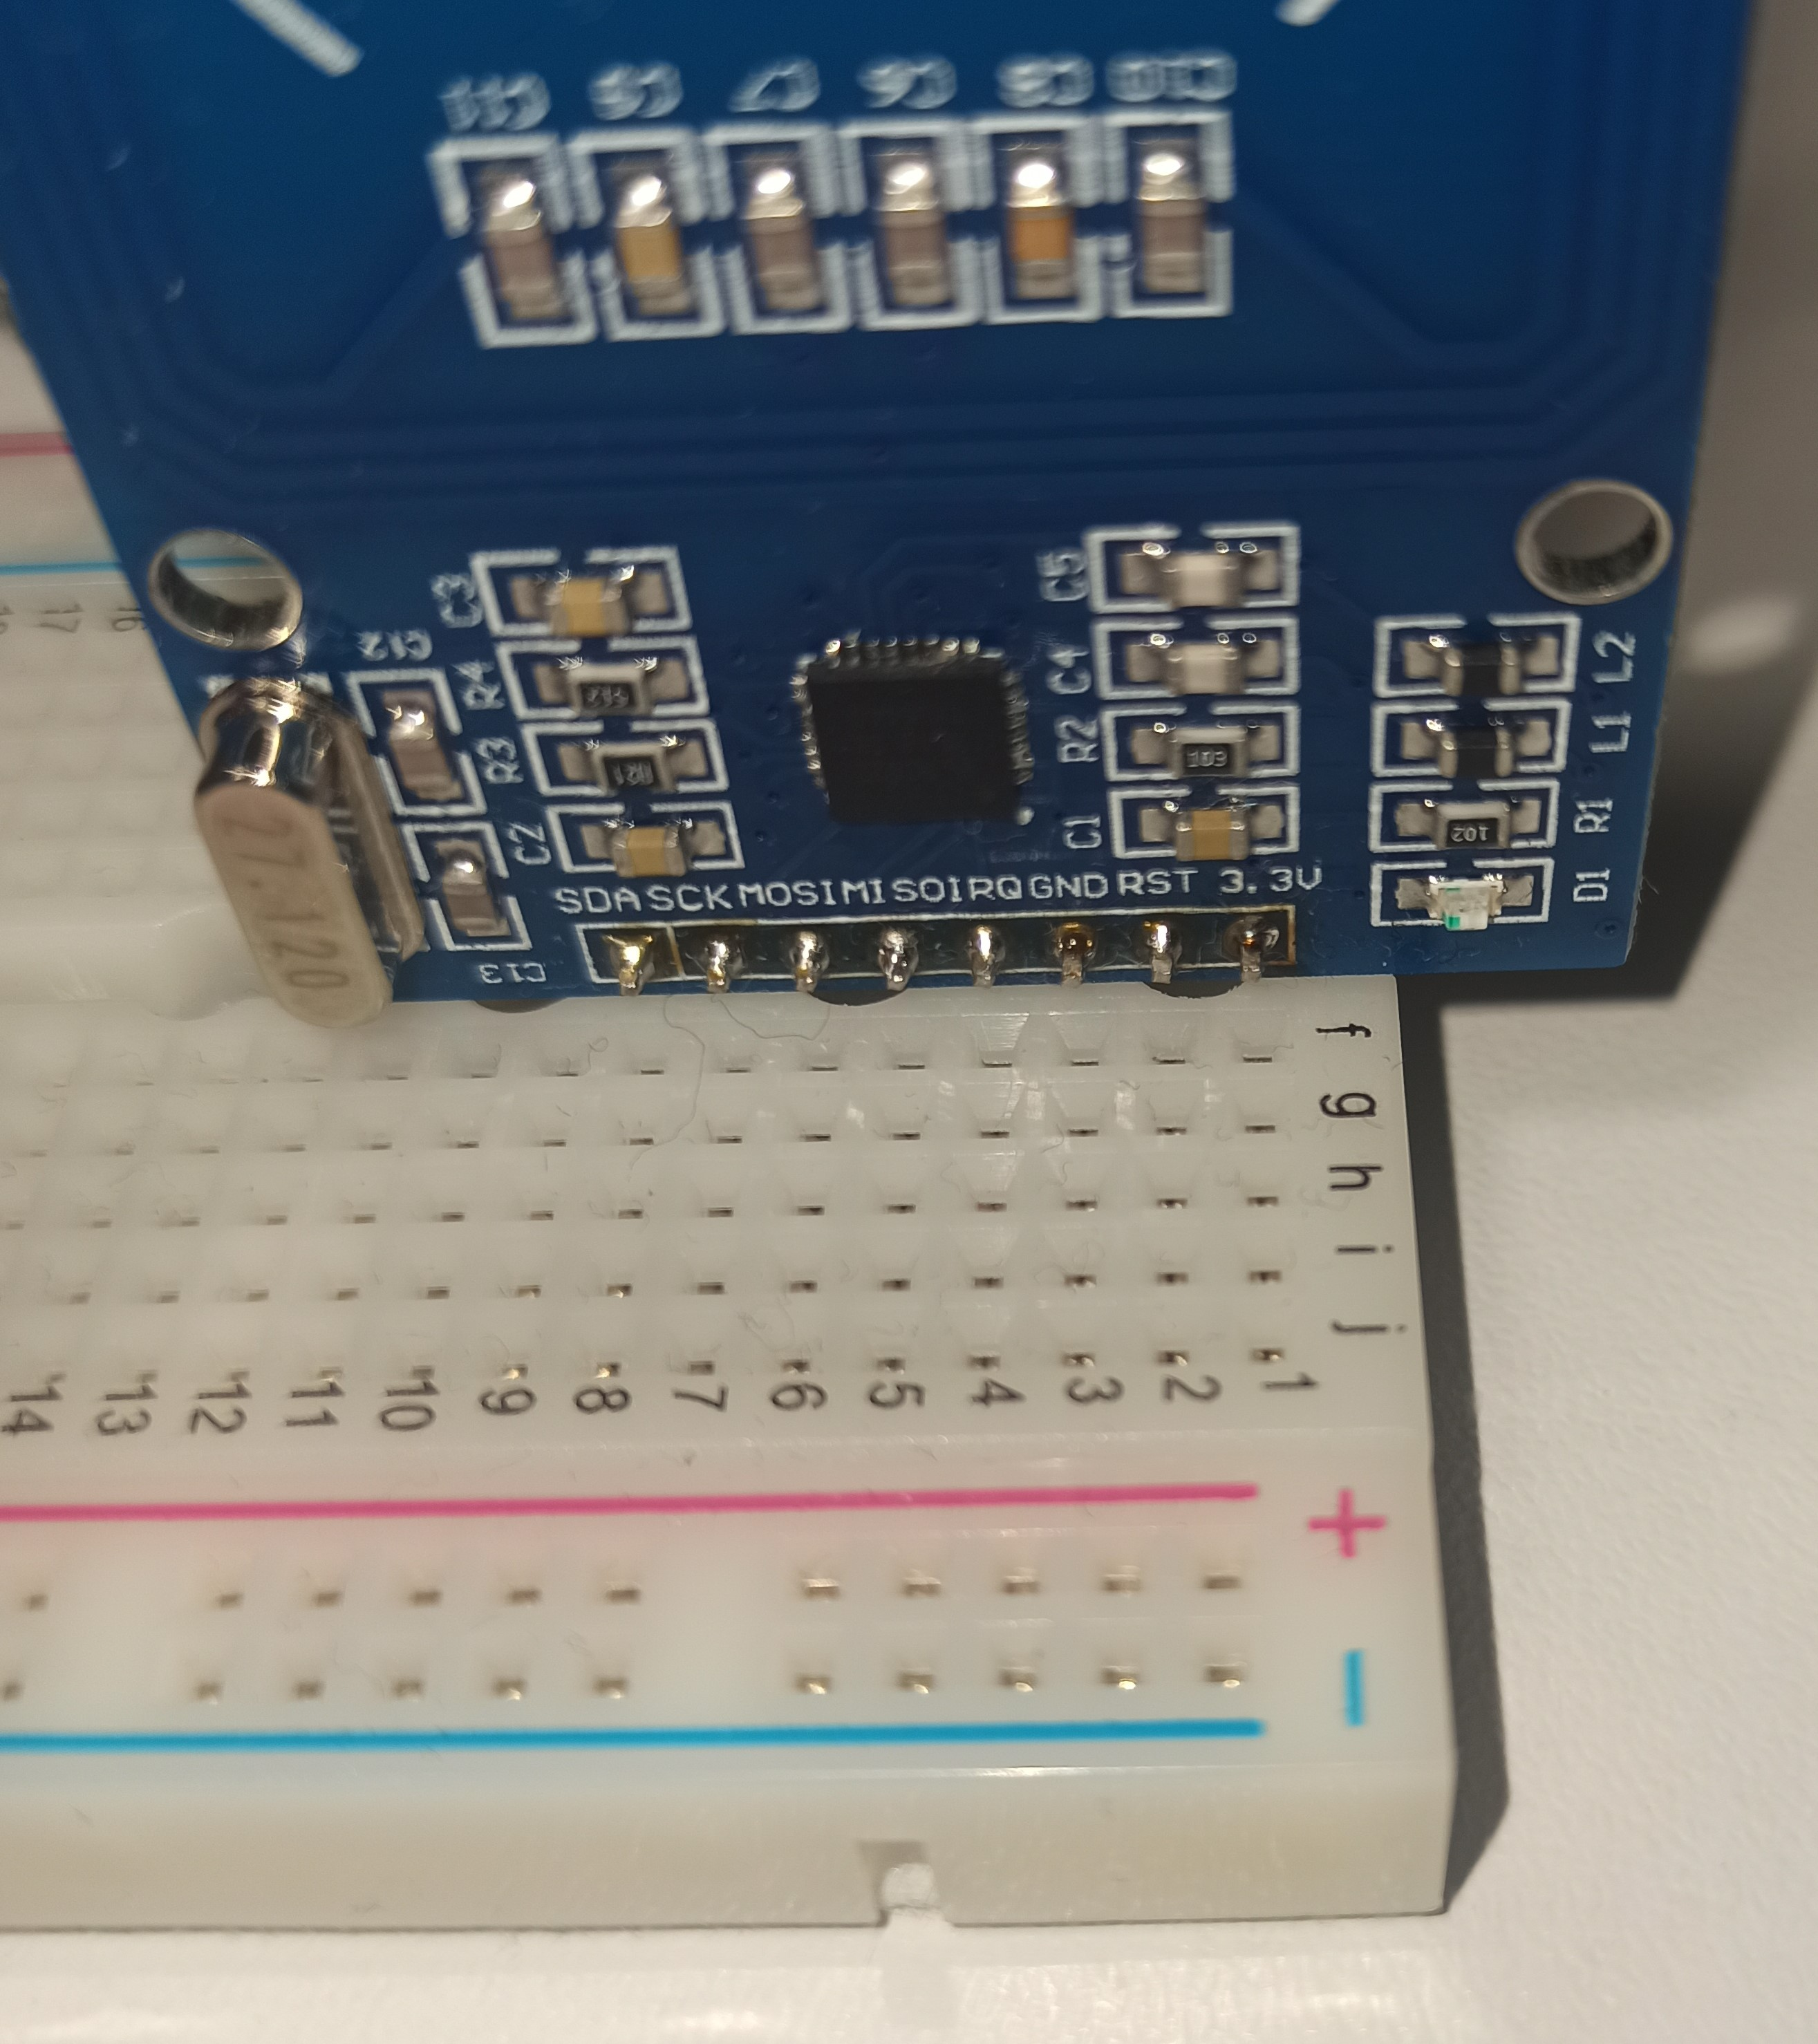
\includegraphics[scale=0.22]{img/contact_plate_reader.jpg}
    \end{center}

    \newpage

    Kolejnym krokiem będzie odpowiednie wpięcie męsko-męskich przewodów połączeniowych w płytkę stykową oraz w płytkę STM.

    Odpowiednie połączenie przedstawione jest w poniższej tabelce:

    \begin{center}
        \begin{tabular}{ |c|c| }
            \hline
            Numer wiersza z płytki stykowej & Pin z płytki STM \\
            \hline
            1 & 3v3 \\
            \hline
            3 & GND \\
            \hline
            5 & A1 \\
            \hline
            6 & A2 \\
            \hline
            7 & D13 \\
            \hline
            8 & D10 \\
            \hline
        \end{tabular}
    \end{center}

    \subsection{Uruchomienie projektu}

    Kolejnymi krokami jakie trzeba podjąć jest uruchomienie projektu - jego kompilacja i wgranie na płytkę STM.

    Aby tego dokonać, należy uruchomić terminal w wybranym folderze, a następnie wykonać komendę:

    \begin{verbatim}
        git clone https://github.com/jakubowiczish/slick_rfid.git
    \end{verbatim}

    W owym katalogu klikamy 2 razy lewym przyciskiem myszy na plik o nazwie: ".project". Nasze uprzednio zainstalowane środowisko powinno się uruchomić.

    Następnie powinniśmy podpiąć płytkę STM do komputera przy użyciu kabla Mini USB.

    W uruchomionym środowisku należy kierować się krokami przedstawionymi na obrazku poniżej:

    \begin{center}
        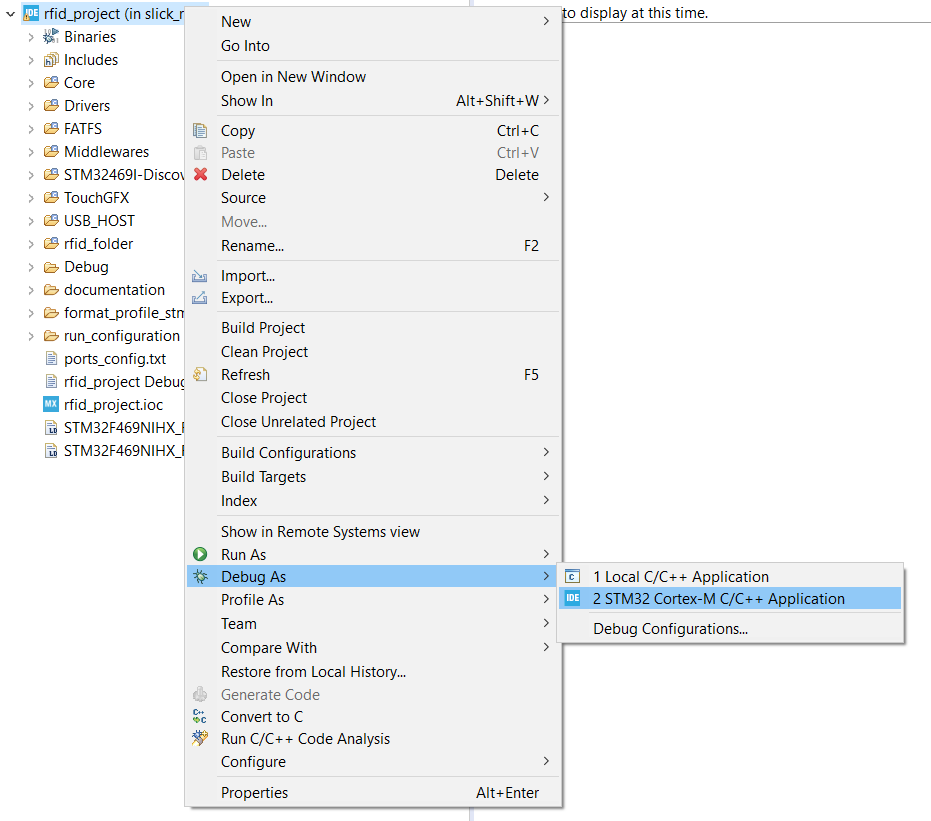
\includegraphics[scale=0.5]{img/run_project.png}
    \end{center}

    Jeśli wszystko przebiegnie pomyślnie, na płytce pojawią się pierwsze instrukcje dla użytkownika.

    \newpage

    \subsection{Korzystanie z czytnika}
    Po wgraniu programu na płytkę można rozpocząć korzystanie z interfejsu.

    \subsubsection{Pierwszy ekran}
    Pierwszym ekranem po uruchomieniu płytki jest ekran, który zachęca nas do przyłożenia naszej karty do czytnika.

    Na płytce prezentuje się on następująco:
    \begin{center}
        
\includegraphics[scale=0.75]{img/screen1.png}
    \end{center}

    Sugeruje on nam, że powinniśmy przyłożyć kartę do czytnika.

    \newpage
    \subsubsection{Drugi ekran}
    Po przyłożeniu naszej karty do czytnika (gdy nie wystąpi żaden błąd) zostajemy przeniesieni do kolejnego ekranu, na którym zostaną wyświetlone dalsze informacje:

    \begin{center}
        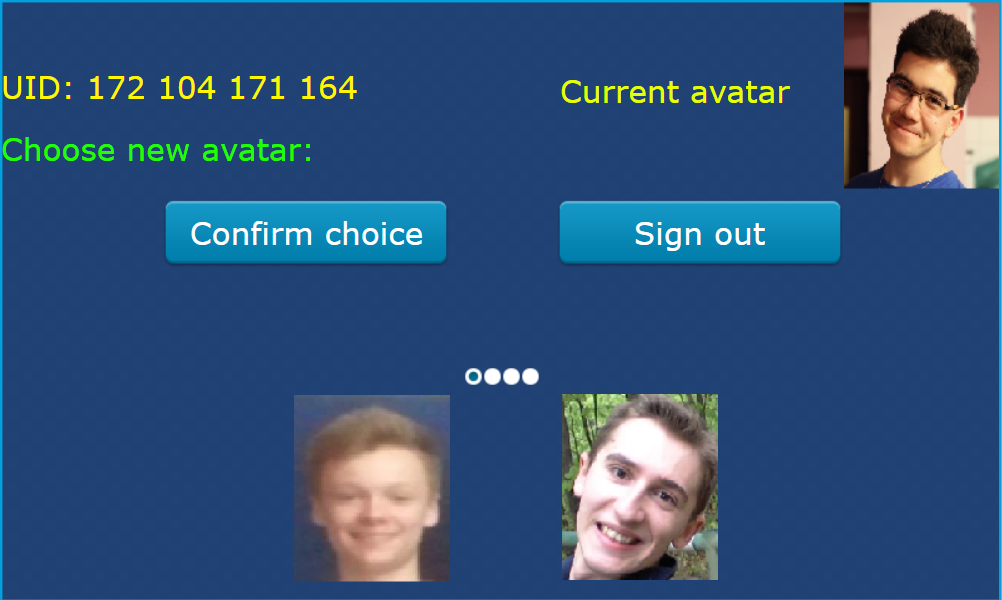
\includegraphics[scale=0.75]{img/screen2.png}
    \end{center}

    Gdy natomiast wystąpi jakaś komplikacja związana z odczytem danych z karty, pozostaniemy na pierwszym ekranie.

    \newpage

    \subsubsubsection{UID}
    Na ekranie płytki możemy ujrzeć różne, zczytane z płytki wartości:

    W lewym górnym rogu zostaje wyświelone UID karty

    \begin{center}
        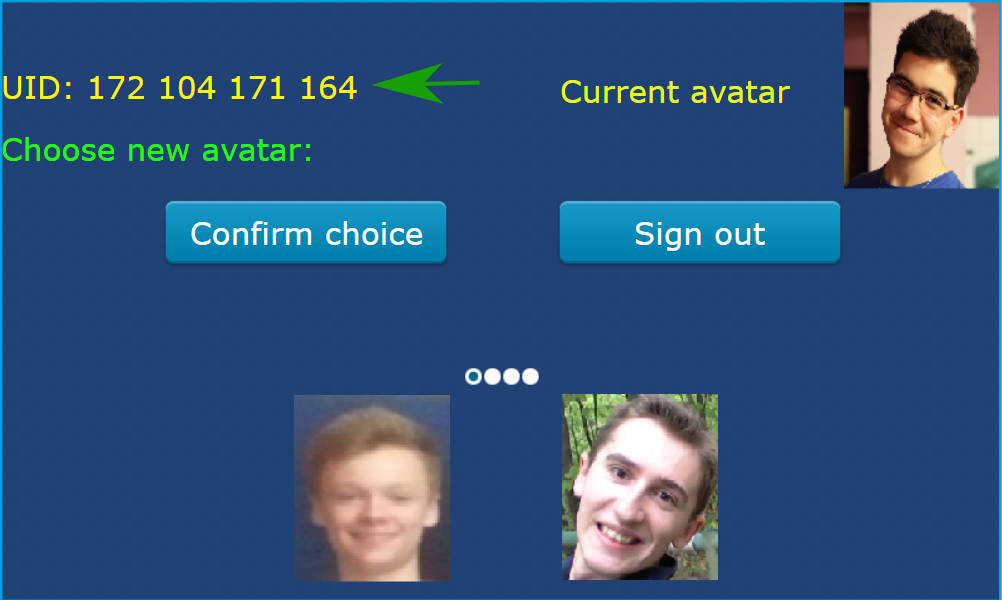
\includegraphics[scale=0.6]{img/screen2-highlighted-uid.png}
    \end{center}

    \subsubsubsection{Avatar}
    W prawym górnym rogu zostaje wyświetlony nasz aktualny avatar

    \begin{center}
        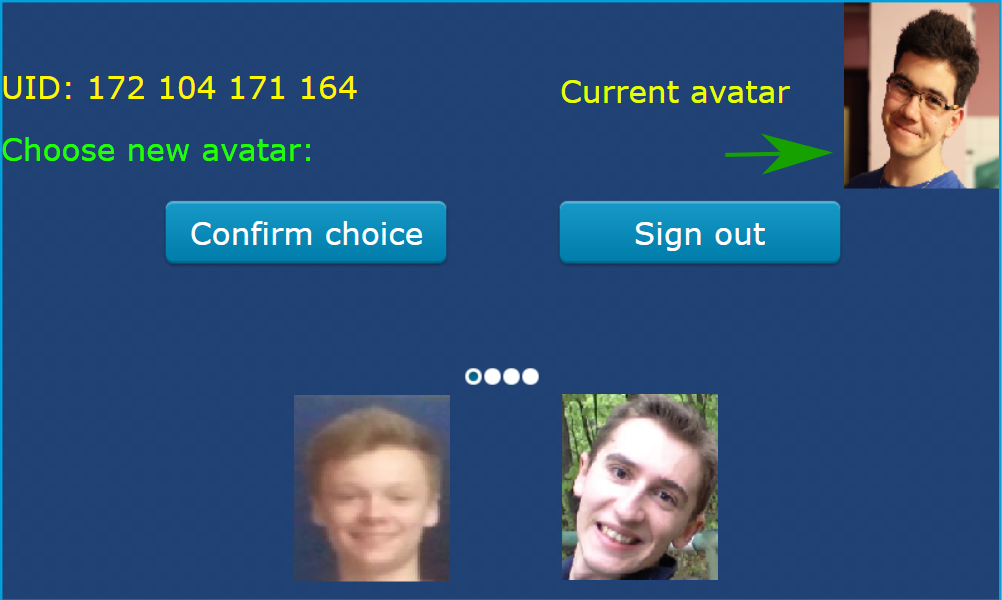
\includegraphics[scale=0.6]{img/screen2-highlighted-avatar.png}
    \end{center}

    \newpage

    \subsubsubsection{Informacja o klikniętym avatarze}
    Obecny widok zawiera również komunikat o tym, aby wybrać nowy avatar, który będzie aktualizowany zaraz po kliknięciu avatara z panelu poniżej:

    \begin{center}
        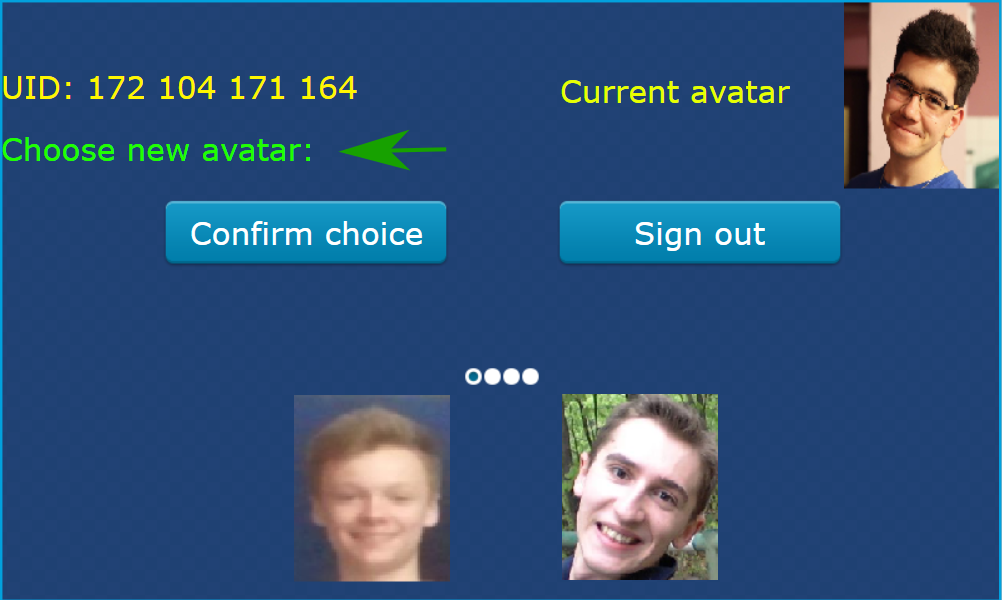
\includegraphics[scale=0.6]{img/screen2-highlighted-choose-empty.png}
    \end{center}

    Gdy klikniemy na jakikolwiek avatar, zostaniemy o tym poinformowani:

    \begin{center}
        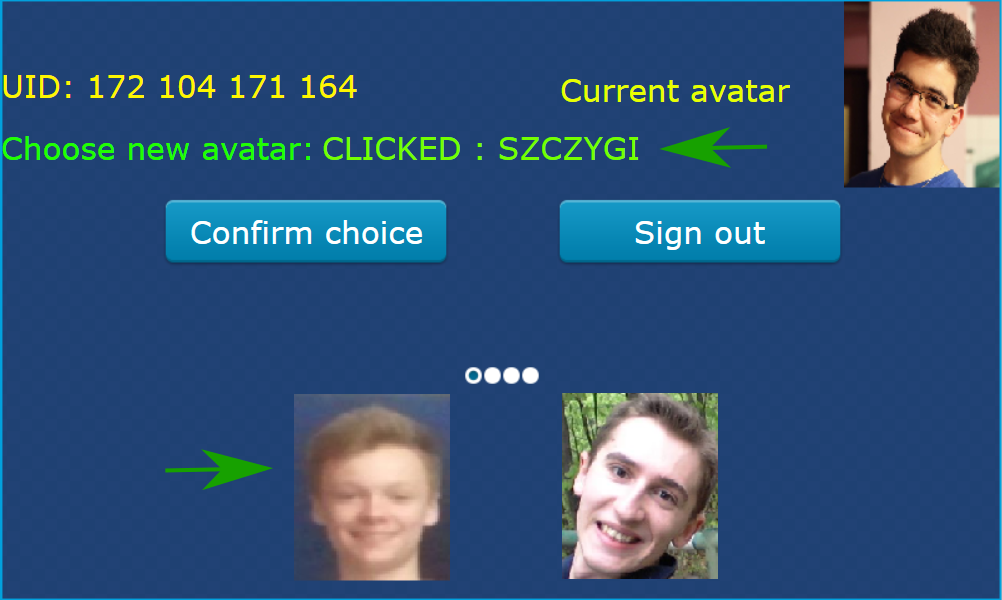
\includegraphics[scale=0.6]{img/screen2-highlighted-avatar-clicked.png}
    \end{center}

    \newpage

    \subsubsubsection{Avatary do wyboru}
    Do wyboru jest 8 avatarów, każdy jest unikalny, posiada inny identyfikator i inną nazwę.

    Aby wybrać odpowiedni avatar, możemy się poruszać się w dolnym pasku na 4 różnych stronach:

    Strona 1
    \begin{center}
        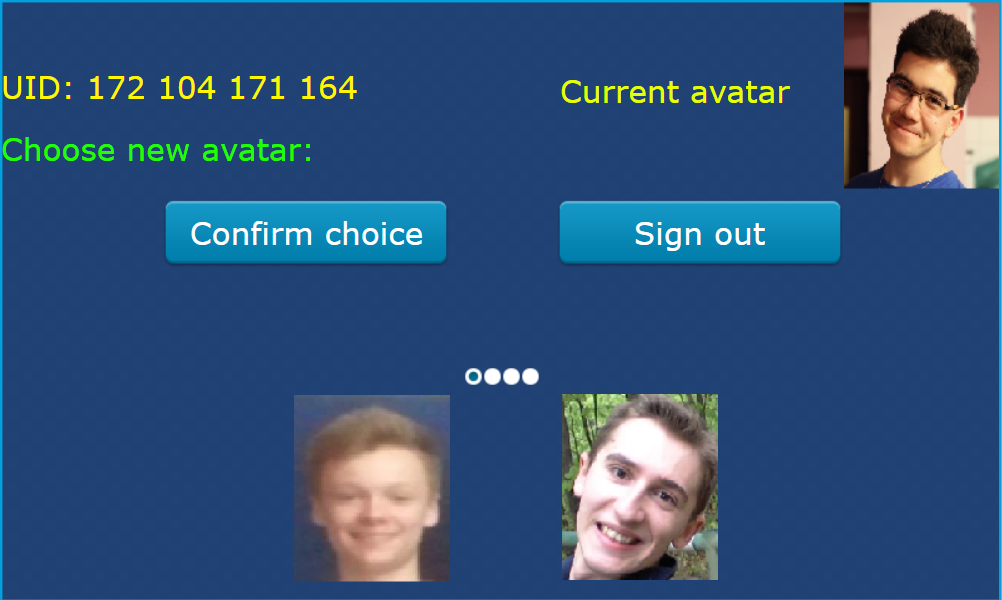
\includegraphics[scale=0.75]{img/screen2-page1.png}
    \end{center}

    Strona 2
    \begin{center}
        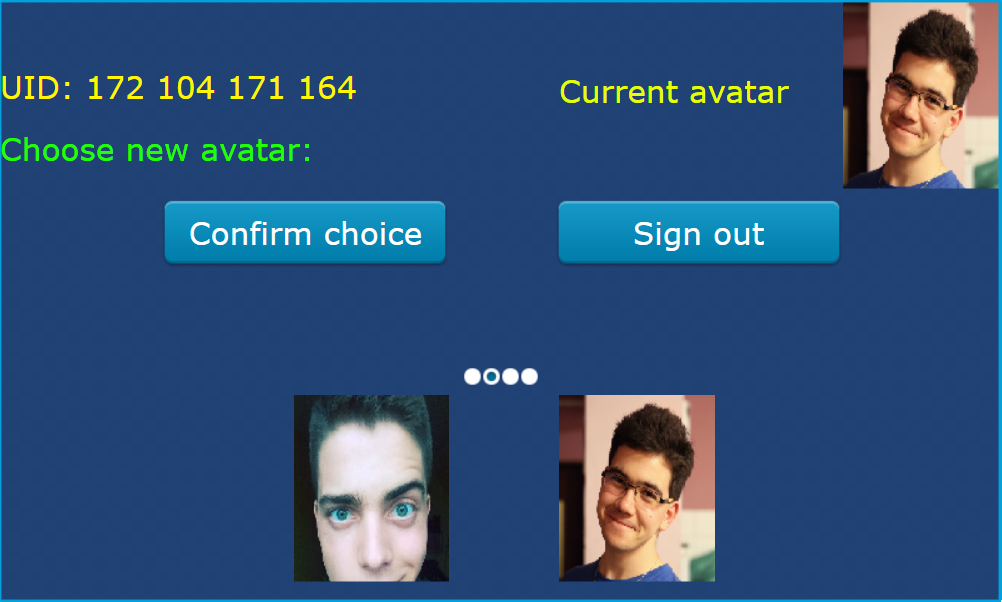
\includegraphics[scale=0.75]{img/screen2-page2.png}
    \end{center}

    \newpage
    Strona 3
    \begin{center}
        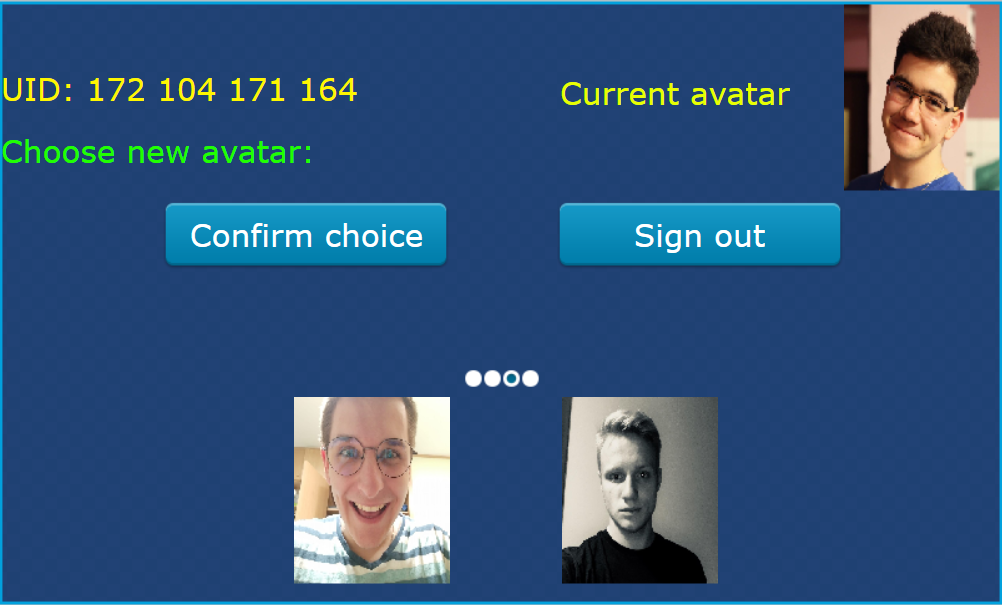
\includegraphics[scale=0.75]{img/screen2-page3.png}
    \end{center}

    Strona 4
    \begin{center}
        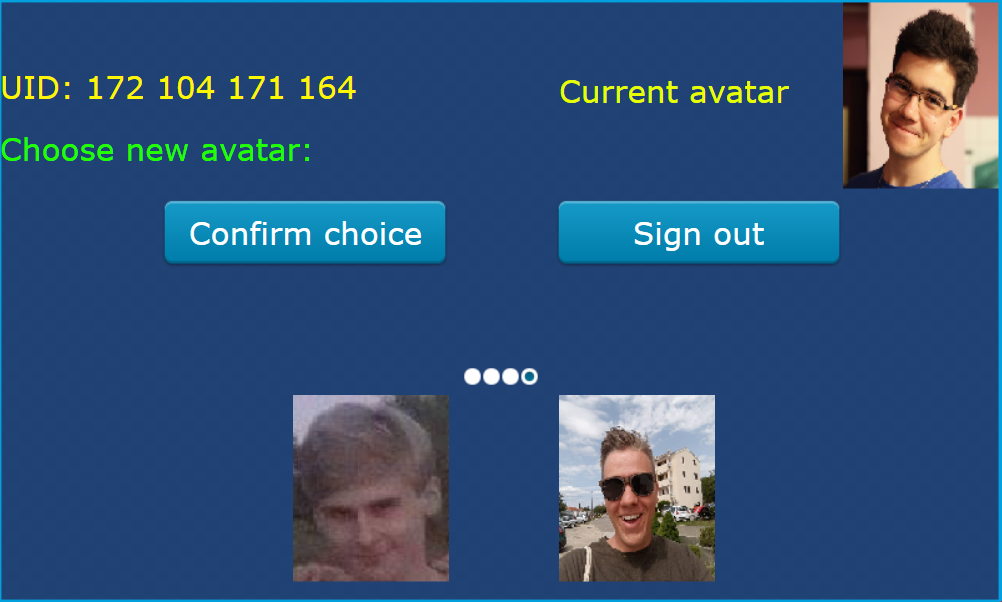
\includegraphics[scale=0.75]{img/screen2-page4.png}
    \end{center}

    \newpage

    \subsubsubsection{Informacja o numerze strony z avatarami}
    Możemy zaobserwować, że widoczny jest wskaźnik oznaczający stronę na której się aktualnie znajdujemy:

    \begin{center}
        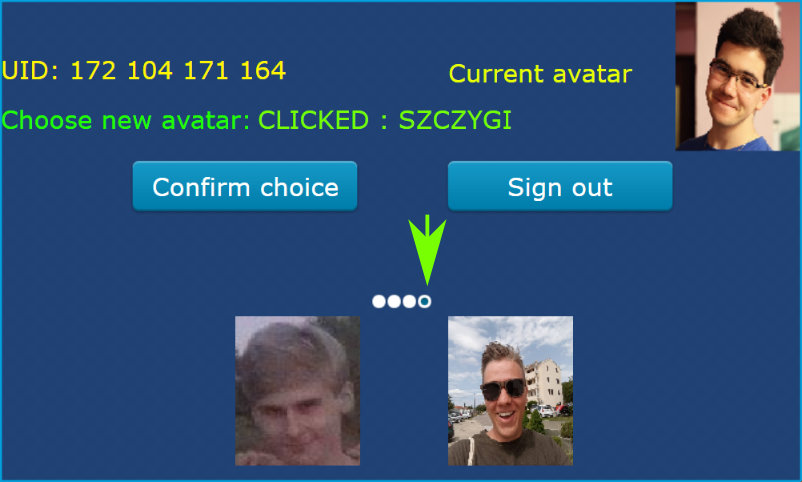
\includegraphics[scale=0.75]{img/screen2-page-indicator.png}
    \end{center}

    \subsubsubsection{Potwierdzenie wyboru avatara}

    Aby dokonać wyboru avatara, musimy najpierw go kliknąć i gdy już uznamy, że jest to nasz ostateczny wybór, klikamy przycisk z napisem "Confirm choice":

    \begin{center}
        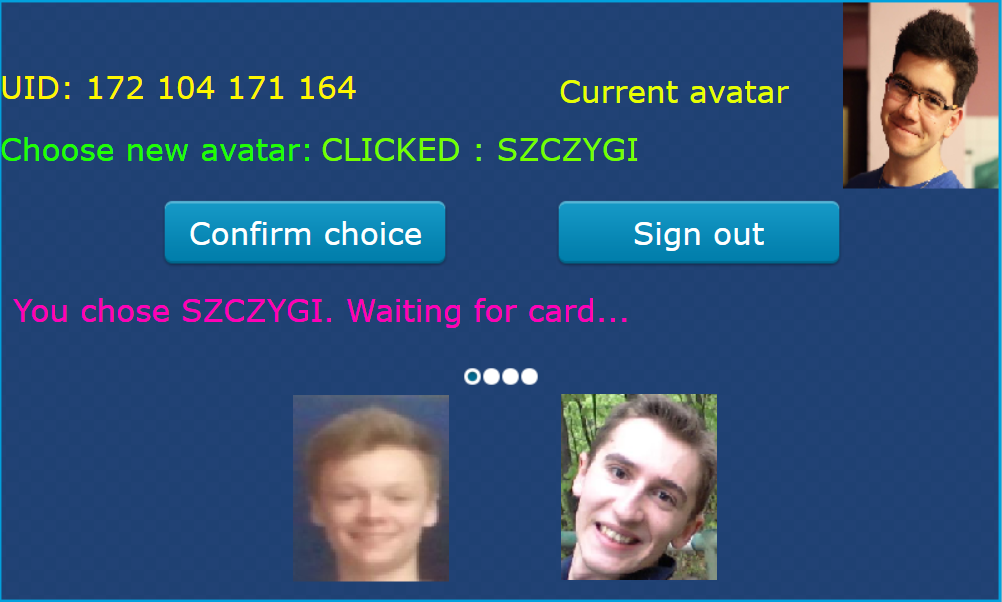
\includegraphics[scale=0.75]{img/screen2-choice-confirmed.png}
    \end{center}

    \subsubsubsection{Zapis danych na kartę}
    Następnie czytnik czeka, aż przyłożymy kartę aby dokonać na nią zapisu naszego wyboru.

    Gdy już to zrobimy, zostaniemy poinformowani o aktualizacji statusu:

    \begin{center}
        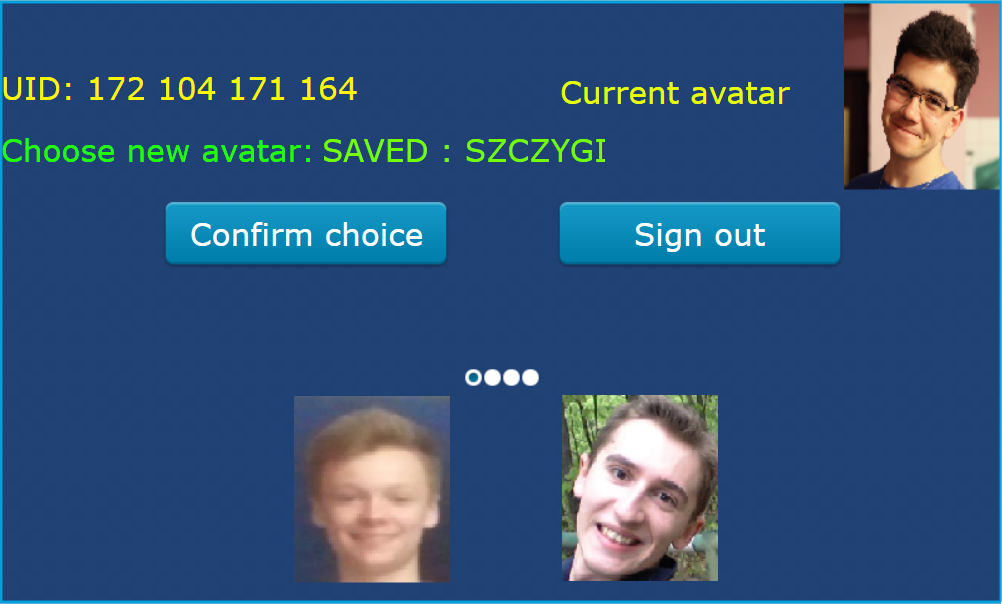
\includegraphics[scale=0.75]{img/screen2-saved.png}
    \end{center}

    \newpage
    \subsubsubsection{Pojawienie się zaktualizowanego avatara}
    Po zapisie danych na kartę dalej będzie jednak będzie widoczny stary avatar.

    Aby ujrzeć nasz nowy avatar, możemy kliknąć przycisk z napisem "Sign out". Możemy również zresetować płytkę.

    Zostaniemy z powrotem przeniesieni na pierwszy ekran i ponownie poproszeni o przyłożenie karty:

    \begin{center}
        
\includegraphics[scale=0.75]{img/screen1.png}
    \end{center}

    Następnie zostaniemy przeniesieni na kolejny ekran, ale naszym oczom ukaże się już zaktualizowany avatar:

    \begin{center}
        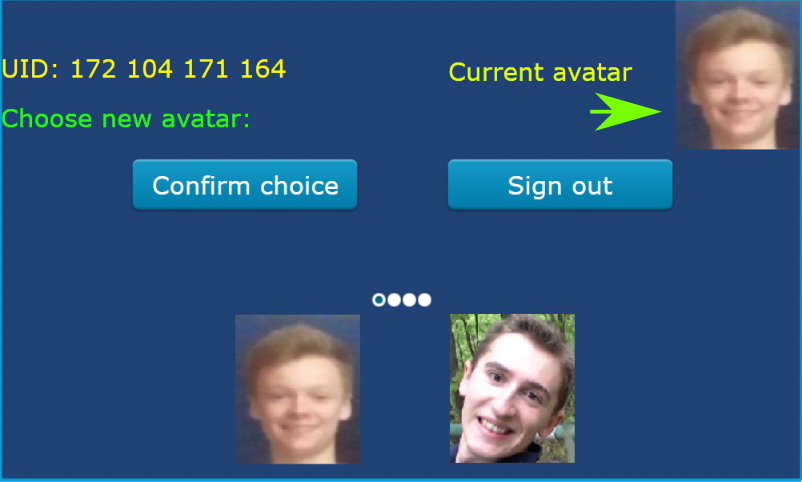
\includegraphics[scale=0.75]{img/screen2-again.png}
    \end{center}
    \vspace{-1.5mm}

    \newpage

    %%%%%%%%%%%%%%%%%%%%%%%%%%%%%%%%%%%%%%%%%%%%%%%%%%%%%%%%%%%%%

    \section{Instrukcja dla planujących rozwijać projekt}
    \vspace{10.5cm}

    Projekt został podzielony na dwa moduły:
    \begin{itemize}
        \item rfid - część odpowiedzialna za komunikację z czytnikiem kard rfid,
        \item TouchGFX - moduł związany z interfejsem użytkownika
    \end{itemize}

    \subsection{Opis funkcji dostępnych w pliku rfid.h}

    \subsubsection{rfid\_configure}
    Funkcja wywoływana na początku działania programu, służy do inicjalizacji odpowiednich pinów i portów GPIO, niezbędnych do działania czytnika kart.
    \inputminted[linenos=true]{c++}{rfid_code/rfid_configure.c}

    \subsubsection{rfid\_init}
    Funkcja, którą należy wykonać po inicjalizacji pinów. Służy do wpisania do rejestrów czytnika kart, odpowiednich wartości inicjalizujących. Oto Kilka ważniejszych wpisów w rejestry:
    \begin{itemize}
        \item przeprowadzenie resetu wszystkich rejestrów,
        \item ustawienie mocy anteny: 48dB
        \item włączenie anteny
    \end{itemize}
    \inputminted[linenos=true]{c++}{rfid_code/rfid_init.c}


    \subsubsection{rfid\_reset}
    Funkcja wywoływana przez rfid\_configure(), dokonuje resetu czytnika.
    \inputminted[linenos=true]{c++}{rfid_code/rfid_reset.c}

    \subsubsection{rfid\_antenna\_on}
    Funkcja wywoływana przez rfid\_configure(), włącza antenę.
    \inputminted[linenos=true]{c++}{rfid_code/rfid_antenna_on.c}


    \subsubsection{rfid\_self\_test}
    Funkcja, która przeprowadza test działania czytnika, poprzez wpisanie w odpowiednie rejestry wartości, oraz wpisanie 25 zer w kolejkę fifo. Po przeprowadzeniu testu, w kolejce fifo dostajemy informację o wersji czytnika rfid oraz kolejne liczby zgodne z dokumentacją. Tak wygląda zawartość kolejki fifo, gdy test się powiedzie:
    \begin{minted}{python}
        00h, EBh, 66h, BAh, 57h, BFh, 23h, 95h,
        D0h, E3h, 0Dh, 3Dh, 27h, 89h, 5Ch, DEh,
        9Dh, 3Bh, A7h, 00h, 21h, 5Bh, 89h, 82h,
        51h, 3Ah, EBh, 02h, 0Ch, A5h, 00h, 49h,
        7Ch, 84h, 4Dh, B3h, CCh, D2h, 1Bh, 81h,
        5Dh, 48h, 76h, D5h, 71h, 061h, 21h, A9h,
        86h, 96h, 83h, 38h, CFh, 9Dh, 5Bh, 6Dh,
        DCh, 15h, BAh, 3Eh, 7Dh, 95h, 03Bh, 2Fh
    \end{minted}
    \inputminted[linenos=true]{c++}{rfid_code/rfid_self_test.c}

    \subsubsection{rfid\_set\_bit\_mask}
    Funkcja pomocnicza, ustawiająca maskę na obecną zawartość rejestru danego.
    \inputminted[linenos=true]{c++}{rfid_code/rfid_set_bit_mask.c}


    \subsubsection{rfid\_clear\_bit\_mask}
    Funkcja pomocnicza, usuwająca wcześniej ustawioną maskę na wartość rejestru (poprzez maskowanie odwrotności bitowej podanej maski).
    \inputminted[linenos=true]{c++}{rfid_code/rfid_clear_bit_mask.c}

    \subsubsection{rfid\_read\_register}
    Funkcja zwracająca zawartość rejestru o danym adresie. Wewnątrz następuje modyfikacja adresu rejstru na:
    \begin{minted}{c++}
        addr = (addr << 1) | 0x80;
    \end{minted}
    Dopisanie 0x80 do końca adresu mówi rfid, że chcemy czytać dany rejestr (nie pisać).
    \inputminted[linenos=true]{c++}{rfid_code/rfid_read_register.c}


    \subsubsection{rfid\_write\_register}
    Funkcja wpisująca dane do rejstru o podanym adresie. Wewnątrz następuje modyfikacja adresu rejstru na:
    \begin{minted}{c++}
        addr = (addr << 1) & 0x7E;
    \end{minted}
    Dopisanie 0x7E do końca adresu mówi rfid, że chcemy wpisać do danego rejestru (nie z niego czytać).
    \inputminted[linenos=true]{c++}{rfid_code/rfid_write_register.c}



    \subsubsection{rfid\_cs\_write}
    Funkcja zmienia stan pinu CS (Chip Select potrzebny do działania SPI) na wysoki lub niski. Jest ona wywoływana przez funkcje rfid\_read\_register oraz rfid\_write\_register. \newline
    Ustawienie na stan niski:
    \begin{minted}{c++}
        rfid_cs_write(GPIO_PIN_RESET);
    \end{minted}
    Ustawienie na stan wysoki:
    \begin{minted}{c++}
        rfid_cs_write(GPIO_PIN_SET);
    \end{minted}
    \inputminted[linenos=true]{c++}{rfid_code/rfid_cs_write.c}

    \subsubsection{rfid\_set\_gain}
    Ustawia zysk energetyczny anteny (antenna gain). Im większą wartość przekaże się do funkcji, z tym większej odległości będzie można czytać karty. Wartość maksymalna to 0xff. Zysk energetyczny jest ustawiany na maksymalny poprzez funkcję rfid\_init.
    \inputminted[linenos=true]{c++}{rfid_code/rfid_set_gain.c}

    \subsubsection{rfid\_get\_gain}
    Zwraca obecnie ustawiony zysk energetyczny anteny (antenna gain).
    \inputminted[linenos=true]{c++}{rfid_code/rfid_get_gain.c}


    \subsubsection{rfid\_read\_version}
    Zwraca wersję odbiornika. Możliwe są dwie wartości:
    \begin{itemize}
        \item 0x91: wersja 1.0
        \item 0x92: wersja 2.0
    \end{itemize}
    \inputminted[linenos=true]{c++}{rfid_code/rfid_read_version.c}

    \subsubsection{rfid\_reqa\_or\_wupa}
    Wysyła do karty komendę REQA lub WUPA. Zgodnie z dokumentacją, aby zacząć komunikację z kartą, trzeba wysłać do niej jedną z tych dwóch komend.
    \inputminted[linenos=true]{c++}{rfid_code/rfid_reqa_or_wupa.c}

    \subsubsection{rfid\_reqa}
    Wysyła do karty komendę REQA. Pod spodem wywołuje funkcję rfid\_reqa\_or\_wupa. W projekcie jest używana tylko komenda REQA, rozpoczynająca komunikację z kartą, więc stworzona została ta funkcja pomocnicza.
    \inputminted[linenos=true]{c++}{rfid_code/rfid_reqa.c}



    \subsubsection{rfid\_to\_card}
    Funkcja zapewniająca komunikację z kartą. Jest wykorzystywana przez wszystkie funkcje chcące komunikować się z kartą.Jej argumenty:
    \begin{itemize}
        \item command - komenda dla czytnika rfid. Zazwyczaj CMD\_TRANSCEIVE, wtedy czytnik wysła dane do karty i czeka na odpowiedź,
        \item waitIRq - bajt używany do sprawdzenia czy poprawnie wykonano komendę. Np dla CMD\_TRANSCEIVE, jest to 0x30,
        \item *send\_data - dane do wysłania do karty,
        \item send\_len - rozmiar tablicy send\_data,
        \item *back\_data - tablica wypełniana bajtami zwróconymi jako odpowiedź z karty,
        \item *back\_len - rozmiar tablicy back\_data, ustawiany przy odbiorze.
        \item *valid\_bits - nie koniecznie zwrócony zostanie nam pełny bajt, jest to ilość bitów ostatniego bajtu jaką należy barć pod uwagę,
        \item rx\_align - ustawia od jakiego bitu wpisywane będą wartości do tablicy *back\_data; zazwyczaj 0,
        \item check\_CRC - jeśli true, sprawdza czy suma kontrolna złożona z dwóch ostatnich bajtów *back\_data się zgadza.
    \end{itemize}

    \inputminted[linenos=true]{c++}{rfid_code/rfid_to_card.c}

    \subsubsection{rfid\_transcive\_data}
    Funkcja pomocnicza wywołująca rfid\_to\_card z command ustawionym na CMD\_TRANSCEIVE oraz z waitIRq ustawionym na 0x30. Pozostałe argumenty takie same jak w przypadku funkcji rfid\_to\_card.
    \inputminted[linenos=true]{c++}{rfid_code/rfid_transcive_data.c}

    \subsubsection{rfid\_calc\_crc}
    Oblicza sumę kontrolną CRC podanej tablicy. Korzysta z gotowych mechanizmów dostarczonych przez czytnik rfid, wpisuje do odpowiednich rejestrów i do kolejki fifo dane. Czytnik rfid sam oblicza sumę kontrolną i sprawdza czy się zgadza.
    \inputminted[linenos=true]{c++}{rfid_code/rfid_calc_crc.c}

    \subsubsection{rfid\_select\_tag}
    Dokonuje wyboru karty, jako tej, z której będzie następowała później komunikacja. Funkcja ta czyta kolejne bity zwracane przez kartę, w tym jej numer UID (identyfikator), SAK (Select Acknowledge). Dodatkowo sprawdza czy zgadza się suma kontrolna CRC. Jeśli wszystko się powiedzie:
    \begin{itemize}
        \item zwracany jest status MI\_OK,
        \item w podanej jako parametr tablicy uid\_tab zapisywany jest UID karty,
        \item w size znajduje się wielkość UID karty (czyli 4, bo tylko takie karty obsługujemy),
        \item w sak znajduje się kod zależny od typu karty. Dla testowych kart było to 0x08.
    \end{itemize}
    \inputminted[linenos=true]{c++}{rfid_code/rfid_select_tag.c}

    \subsubsection{rfid\_authenticate}
    Wysyła do karty komendę autentykacji. Dzięki niej można pisać / czytać zawartość karty. Jej argumenty to:
    \begin{itemize}
        \item command - MIF\_AUTHENTA jeśli chcemy czytać zwartość karty lub MIF\_AUTHENTB jeśli chcemy wpisywać do karty,
        \item blockAddr - w kartach mifare classic 1k mamy 16 bloków, więc jest to wartośc z przdziału 0 - 15. W bloku 0, w sektorze 0 mamy wpisane UID karty + dodatkowe wartości od producenta, ta część jest nie modyfikowalna - tylko do odczytu.
        \item key - każdy blok jest zabezpieczony kodem, osobny kod w przypadku chęci czytania i osobny do zapisu (w zależności czy w argumencie command podamy MIF\_AUTHENTA czy MIF\_AUTHENTB).
        \item uid - musimy podać tablicę długości 4 bajty, w której znajduje się UID karty. Należy go odczytać wywołując wcześniej funkcję rfid\_select\_tag.
    \end{itemize}
    Funkcję tę należy wykonać dopiero po wywołaniu funkcji rfid\_select\_tag.
    \inputminted[linenos=true]{c++}{rfid_code/rfid_authenticate.c}


    \subsubsection{rfid\_card\_read}
    Czyta dane z wcześniej wybranego bloku przez rfid\_authenticate (0-15) w wybranym sektorze (0-4). Zapisuje do *buffer.
    \inputminted[linenos=true]{c++}{rfid_code/rfid_card_read.c}

    \subsubsection{rfid\_card\_write}
    Wpisuje dane z buffer'a do wcześniej wybranego bloku przez rfid\_authenticate (0-15) w wybranym sektorze (0-4).
    \inputminted[linenos=true]{c++}{rfid_code/rfid_card_write.c}

    \subsubsection{rfid\_card\_transceive}
    Funkcja pomocnicza, służąca do wydawania komend karcie. Wywołuje pod spodem rfid\_transcive\_data, lecz karta wymaga aby na końcu przesyłanej tablicy znajdowała się suma kontrolna CRC, więc dopisuje do danych, które chcemy przesłać sumę kontrolną.
    \inputminted[linenos=true]{c++}{rfid_code/rfid_card_transceive.c}

    \subsubsection{rfid\_is\_new\_card}
    Sprawdza czy jest jakaś karta w zasięgu nadajnika. Wywołuje pod spodem funkcję auth\_a. Jeśli karta jest obecna zwraca true, jeśli nie jest, zwraca false.
    \inputminted[linenos=true]{c++}{rfid_code/rfid_is_new_card.c}

    \subsubsection{rfid\_halt}
    Wysyła do karty wiadomość, o chęci przerwania komunikacji. Karta może teraz znowu być rozpoznawana przez odbiornik.
    \inputminted[linenos=true]{c++}{rfid_code/rfid_halt.c}

    \subsubsection{rfid\_stop\_crypto}
    Po wywołaniu funkcji rfid\_halt, należy wywołać tę funkcję. Czyści ona rejestr i przygotowuje odbiornik do możliwości czytania nowych kart.
    \inputminted[linenos=true]{c++}{rfid_code/rfid_stop_crypto.c}

    %%%%%%%%%%%%%%%%%%%%%%%%%%%%%%%%%%%%%%%%%%%%%%%%%%%%%%%%%%%

    \section{Problemy napotkane podczas tworzenia projektu}
    \vspace{10.5cm}

    \subsection{Problemy z konfiguracją projektu w CubeMX}
    Największym problemem była konfiguracja wyświetlacza LCD mikro-kontrolera STM32f4 w CubeMX. Na wyświetlaczu pokazywał się obraz tylko w 1/4 całej powierzchni ekranu. Po przeczytaniu wielu podobnych wątków na forach internetowych związanych z tą właśnie płytką, okazało się, że problem leży w samym programie CubeMX, który źle konfiguruje wyświetlacz konkretnego mikro-kontrolera.
    
    \vskip 0.2in
    Należało więc ręcznie zmienić konfigurację wyświetlacza w plikach źródłowych po generacji kodu. 

    \subsection{Problemy z działaniem portu UART na module RFID RC522}
    Duża część czasu została przeznaczona na próbę nawiązania komunikacji z modułem RFID przy pomocy portu UART, który był wykorzystywany na zajęciach z Techniki Mikroprocesorowej. W dokumentacji modułu, napisane jest, że potrafi on korzystać z UART, lecz próby nawiązania z nim połączenia były bezskuteczne. Ponownie skorzystano z pomocy forów internetowych, gdzie dowiedziano się, że aby port UART działał, należało ręcznie przeciąć połączenie między dwoma stykami na płytce. 
    Zastosowano więc inny port do łączenia z płytką - SPI. Należało również doszkolić się z jego działania i nauczyć się go konfigurować w programie CubeMX.
    

    \subsection{Problemy z aktualizacją komponentów na ekranie płytki}

    \subsubsection{Problem z responsywnością ekranu}

    Aby zapewnić aktualizację danych na ekranie w odpowiednim tempie trzeba było zapewnić odpowiedni flow programu tj. odpowiednie przekazywanie danych z modelu do prezentera i z prezentera do widoku - przy zczytywaniu danych z karty - oraz w drugą stronę - przy zapisywaniu danych na kartę.

    \vskip 0.2in

    Gdy na początku planowane było pominięcie udziału modelu w zapisie danych na kartę, okazało się to problematyczne ponieważ występowały poważne problemy z responsywnością widoku - widok zawieszał się lub przestawał wykonywać nakazane instrukcje.

    \subsubsection{Problem z aktualizowaniem komponentów odpowiedzialnych za zmieniający się tekst na ekranie}

    W przypadku komponentów odpowiedzialnych za pokazywanie zmieniającego się tekstu na ekranie, problemy wystąpiły w przypadku wywołań funkcji odpowiedzialnych za aktualizowanie bufora przechowującego aktualny stan napisu.

    \vskip 0.2in

    Sporo czasu zajęło zrozumienie na czym polegał błąd, ponieważ funkcja aktualizująca bufor odpowiedzialny za przechowywany tekst działała poprawnie tylko dla integerów.

    \vskip 0.2in

    Kluczem do rozwiązania problemu była odpowiednia konwersja napisów typu char* na napisy typu UnicodeChar* - specjalnego typu używanego przez funkcję odpowiedzialną za aktualizację bufora (mimo, że żadne ostrzeżenie ani błędy kompilacji nie występowały).
    
    
    \section{Bibliografia}
    \vspace{10.5cm}
 \begin{itemize}
    
\item \url{https://touchgfx.zendesk.com/hc/en-us/articles/207015345}
    
\item \url{https://touchgfx.zendesk.com/hc/en-us/articles/360018667192-Step-1-Setting-up-the-two-Screens}
    
    \item \url{https://touchgfx.zendesk.com/hc/en-us/articles/205443742-Step-2-Adding-Buttons}
    
    \item \url{https://touchgfx.zendesk.com/hc/en-us/articles/205587571-Step-3-Adding-Text}

    \item \url{https://touchgfx.zendesk.com/hc/en-us/articles/205443982-Step-4-Adding-code}

    \item \url{https://www.nxp.com/docs/en/data-sheet/MFRC522.pdf}
    
    \item \url{https://www.nxp.com/docs/en/data-sheet/MF1S50YYX_V1.pdf}
    
    \item \url{https://forum.arduino.cc/index.php?topic=442750.0}
    
    \item \url{https://community.st.com/s/question/0D50X0000Ay9hWFSQY/touchgfx-cubemx-cubeide-integration-problems-please-help}
 \end{itemize}
\end{document}